%% Beginning of file 'sample.tex'
%%
%% Modified 2005 December 5
%%
%% This is a sample manuscript marked up using the
%% AASTeX v5.x LaTeX 2e macros.

%% The first piece of markup in an AASTeX v5.x document
%% is the \documentclass command. LaTeX will ignore
%% any data that comes before this command.

%% The command below calls the preprint style
%% which will produce a one-column, single-spaced document.
%% Examples of commands for other substyles follow. Uase
%% whichever is most appropriate for your purposes.
%%
%%\documentclass[12pt,preprint]{aastex}
%% manuscript produces a one-column, double-spaced document:

\documentclass[manuscript]{emulateapj}
%\documentclass[manuscript]{aastex}
\usepackage{natbib}

%% preprint2 produces a double-column, single-spaced document:

%% \documentclass[preprint2]{aastex}

%% Sometimes a paper's abstract is too long to fit on the
%% title page in preprint2 mode. When that is the case,
%% use the longabstract style option.

%% \documentclass[preprint2,longabstract]{aastex}

%% If you want to create your own macros, you can do so
%% using \newcommand. Your macros should appear before
%% the \begin{document} command.
%%
%% If you are submitting to a journal that translates manuscripts
%% into SGML, you need to follow certain guidelines when preparing
%% your macros. See the AASTeX v5.x Author Guide
%% for information.

\newcommand{\lsim}{\mbox{$_<\atop^{\sim}$}}
\newcommand{\gsim}{\mbox{$_>\atop^{\sim}$}}
\newcommand{\vdag}{(v)^\dagger}
\newcommand{\myemail}{scarlata@ipac.caltech.edu}
\newcommand{\lya}{Ly$\alpha$}
\newcommand{\ha}{H$\alpha$}
\newcommand{\hb}{H$\beta$}
\newcommand{\hi}{H~{\small I}}
\newcommand{\hii}{H~{\small II}}
\newcommand{\oii}{[O~{\small II}]}
\newcommand{\oiii}{[O~{\small III}]}
\newcommand{\heii}{He~{\small II}}
\newcommand{\civ}{C~{\small IV}}
\newcommand{\ciii}{[C~{\small III]}}
\newcommand{\nii}{[N~{\small II]}}
\newcommand{\tbd}{{\bf TBD}}
\newcommand{\ecsa}{erg cm$^{-2}$ s$^{-1}$ \AA$^{-1}$}
\newcommand{\ecs}{erg cm$^{-2}$ s$^{-1}$}
\newcommand{\es}{erg s$^{-1}$}
\newcommand{\esa}{erg s$^{-1}$}
\newcommand{\kms}{km s$^{-1}$}
\newcommand{\lsimeq}{\mbox{$_<\atop^{\sim}$}}

%% You can insert a short comment on the title page using the command below.

%\slugcomment{Draft}

%% If you wish, you may supply running head information, although
%% this information may be modified by the editorial offices.
%% The left head contains a list of authors,
%% usually a maximum of three (otherwise use et al.).  The right
%% head is a modified title of up to roughly 44 characters.
%% Running heads will not print in the manuscript style.

\shortauthors{Scarlata, C. et al.}

%% This is the end of the preamble.  Indicate the beginning of the
%% paper itself with \begin{document}.
 
\begin{document}

%% LaTeX will automatically break titles if they run longer than
%% one line. However, you may use \\ to force a line break if
%% you desire.

\title{High resolution HST-COS \lya\ profile}

%% Use \author, \affil, and the \and command to format
%% author and affiliation information.
%% Note that \email has replaced the old \authoremail command
%% from AASTeX v4.0. You can use \email to mark an email address
%% anywhere in the paper, not just in the front matter.
%% As in the title, use \\ to force line breaks.

\author{C. Scarlata, J. Colbert, H. I. Teplitz}

\affil{{\it Spitzer} Science Center, California Institute of Technology, 314-6, Pasadena, CA-91125}

\author{N. Panagia\altaffilmark{2,7,9}, M. Hayes\altaffilmark{3}, B. Siana\altaffilmark{4}, A. Rau\altaffilmark{4,5}, P. Francis\altaffilmark{6}, A. Caon\altaffilmark{1,8}, A. Pizzella\altaffilmark{8}, C. Bridge\altaffilmark{1}}

 \altaffiltext{2}{Space Telescope Science Institute, 3700 San Martin Drive, Baltimore, MD 21218, USA}
 \altaffiltext{3}{Observatoire de Geneve, 51, Ch. des Maillettes, CH-1290, Sauverny, Switzerland}
 \altaffiltext{4}{California Institute of Technology, MS 105-24, Pasadena, CA91125}
 \altaffiltext{5}{Max-Planck-Institut f\"ur extraterrestrische Physik, Giessenbachstrasse 1, 85748 Garching, Germany}
 \altaffiltext{6}{Research School of Astronomy and Astrophysics, the Australian National University, Canberra 0200, Australia}
 \altaffiltext{7}{INAF/Osservatorio Astrofisico di Catania, Via S.Sofia 78, I-95123 Catania, Italy}
 \altaffiltext{8}{Department of Astronomy, University of Padova, Vicolo dell'Osservatorio 3, I-35122, Padova, Italy}
 \altaffiltext{9}{Supernova Ltd., Olde Yard Village 131, Northsound Road, Virgin Gorda, British Virgin Islands}

% \altaffiltext{3}{Carnegie Observatories}
%Supernova Ltd., Olde Yard Village #131, Northsound Road, Virgin Gorda, British Virgin Islands}

%ICRANet, Piazzale della Repubblica 10, I-65100 Pescara, Italy
%% Notice that each of these authors has alternate affiliations, which
%% are identified by the \altaffilmark after each name.  Specify alternate
%% affiliation information with \altaffiltext, with one command per each
%% affiliation.


%% Mark off your abstract in the ``abstract'' environment. In the manuscript
%% style, abstract will output a Received/Accepted line after the
%% title and affiliation information. No date will appear since the author
%% does not have this information. The dates will be filled in by the
%% editorial office after submission.

\begin{abstract}
 \end{abstract}

%% Keywords should appear after the \end{abstract} command. The uncommented
%% example has been keyed in ApJ style. See the instructions to authors
%% for the journal to which you are submitting your paper to determine
%% what keyword punctuation is appropriate.

\keywords{galaxies: ISM --- ISM: structure}

\section{Introduction}
We use a standard $H_0 = 70$ km s$^{-1}$ Mpc$^{-1}$, $\Omega_M = 0.3$,
and $\Omega_\Lambda = 0.7$ cosmology.

\section{The sample}
The targets for the HST COS spectroscopic followup are taken from the
sample of \lya\ emitters identified by Deharveng et al.\ (2008) and
Cowie et al.\ (2010) in deep GALEX grism spectroscopy. The GALEX
sample includes 119 \lya\ emitters, 49 of which have rest-frame \lya\
emission line EW $>20$\AA.  From the parent sample of GALEX \lya\
emitters, we originally selected 25 galaxies that satisfied the
following criteria: 1) are classified as star-forming based on optical
emission line ratios (e.g., Cowie et al. 2010), 2) have \lya\ emission
line rest--frame EW$>20$~\AA\ in the low resolution GALEX spectra, and
3) have redshift confirmed using optical spectroscopy.  As we show in
Scarlata et al.\ (2009), Atek et al.\ (2009), Finkelstein et
al. (2009), and Cowie et al.\ (2010), the requirement of having the
optical confirmation does not change the target selection function of
the sample, since 100\% of the sources we followed up were, in fact,
confirmed.  % Focusing here on the \lya\ emission-line profile in
% star-forming galaxies, we removed those emitters with optical line
  % ratios consistent with an AGN, using the Baldwin, Phillips, \&
% Terlevich (BPT, 1981) diagram. 
High redshift \lya\ emitters are usually selected with Hu et al.'s
(1998) definition that they have a rest frame EW greater than
$20$~\AA\ (see also Kornei et al. 2010). Thus, the EW cut ensures that
we are able to make a valid comparison with the samples of \lya\
emitters selected at $z>2$. 

\citet{deharveng2008} identified broad-line AGN in their sample of
\lya\ emitters as those objects with \lya\ line widths broader than
1200 \kms. Narrow line AGN could not be identified since other
diagnostic lines of AGN activity % (such as \civ\ and \ciii)
were either too faint, or fell in a noisy part of the UV spectra.  In
order to identify the narrow line AGN, we have used the classic
\citet[][BPT]{baldwin1981} diagram of \oiii/\hb\ versus \nii/\ha
(shown in Figure~\ref{fig:agn}).

% The theoretical maximum line ratios possible for pure stellar
% photoionization are shown as a dashed curve in Figure~\ref{fig:agn}
% \citep{kewley2001}. To be conservative, we use the
% \citet{kauffmann2003} empirical separation between active and
% star-forming galaxies (solid line). We find that in 2 of our \lya\
% emitters the gas is likely to be ionized by an active nucleus. We note
% that both cases are in the region of the diagram where stellar
% photoionization cannot be excluded on the basis of theoretical
% calculations \citep{kewley2001}.  Among the six galaxies that could
% not be placed on the BPT diagram, we could still classify 5 of them
% using either \nii/\ha\ ratio, or the line width. We identify the AGN
% as those galaxies for which $\log \left( [N~II] / H~\alpha \right)
% \geq -0.4$ \citep{miller2003,carter2001}.  We add 2 AGN based on the
% \nii/\ha\ ratio.  Finally, one of the two galaxies for which the \ha\
% is too red to be covered by our spectrum has an \oiii\ line width
% typical of an AGN ($\sim 1090$ \kms). To summarize, we identify 5 AGN
% out of a sample of 30 galaxies, i.e, the fraction of \lya\ emitters
% classified as AGN is 17\%, consistent with the recent measurement by
% \citep[][15\%]{cowie2009}, and marginally consistent with the
% measurement by \citet[][43$^{+18}_{-26}\%$]{finkelsteinagn}. However,
% Finkelstein et al. (2009) classify AGN using also the presence of high
% ionization emission lines, that may be indicative of a high-excitation
% star forming galaxy, rather than an active nucleus.

% In the following analysis we only consider those 20 galaxies that are
% classified as star-forming, and with {\it both} \ha\ and \hb\ detected
% in the spectrum.


% The proposed target GALEX \lya\ emitters
% stand as the first unbiased and statistically meaningful sample of
% \lya\ emitting galaxies at low redshift.

\section{Observations and data analysis}
\label{sec:data}
The galaxies were observed between February and October 2011, with the
COS FUV, medium-resolution G160 grism. Each galaxy was observed for 1
orbit. For 22 out of the 25 galaxies, the imaging target acquisition
was performed on a star close to the science target (distance $\le
2$'). The telescope was then offset to center the COS aperture on the
science target. The offsets were computed from ground based images in
most cases, while ACS HST imaging was used for the objects in the
COSMOS field (see Table~\ref{tab:info}). In order to check the
acquisition procedure, we obtained a direct NUV image after the
telescope was shifted to te target position.  The exposure times of
the images vary between 80 and 200 seconds, depending on the GALEX NUV
magnitude of the target. The remaining of each orbit was used for the
spectroscopic observations in TIME-TAG mode, with typical exposure
times of 2300s.  We chose the grism central wavelength to ensure that
the \lya\ would not fall in the wavelength gaps due to the physical
layout of the detectors and the optics. In order to minimize the
impact of microchannel plate detector fixed pattern noise, we took two
exposures for each target, with FP-POS$=3$ and FP-POS$=4$,
respectively. The wavelength range covered by the COS spectra is
approximately $1405-1775$\AA, with a dispersion of 12.23\AA\
px$^{-1}$. 
                        
We recalibrated and re-extracted the COS spectra using {\tt calcos}
v2.15.4 task in pyraf. Due to the target acquisition strategy, the
galaxies were not perfectly centered in the COS aperture. We used the
direct NUV images to measure the shifts in the dispersion direction
between the position of the center of each galaxy and the expected
position of the COS aperture center. The shifts ranged between $-19$
and 10 NUV pixels, with a standard deviation of 8 pixels
(corresponding to 0.1\AA). The correction to the wavelength zero
point was applied to the wavelength column in the {\tt corrtag} files,
and {\tt calcos} was the run again with the edited files as
input. This correction does not only take care of the wavelength zero
point, but also allows us to apply the proper sensitivity at each
wavelength.

The PSA aperture throughput decreases toward the edges of the field of
view, due to the increasing vignetting of the flux. This change in
throughput is not accounted for in the {\tt calcos} pipeline,
resulting in an underestimate of the extracted flux for extended
sources. We scaled the extracted spectra by a correction factor
computed using the directing imaging, and assuming that the aperture
throughput is symmetric with respect to the aperture center. The
scaling factors vary between 1.15 and 1.45, for the most compact and
most extended sources, respectively. In Figure~\ref{fig:GALEX_COSflux}
we compare the total aperture corrected NUV flux measured from the COS
images within the 2\farcs5 aperture with the GALEX NUV total flux. The
fluxes in the smaller COS apertures are systematically lower than the
GALEX fluxes, indicating that 

For four galaxies (see Table~\ref{tab:sample}) the star used for the
acquisition was too bright to be observed with MIRRORA. We then
performed the acquisition using MIRRORB and moved to MIRRORA for the
science exposures. Although the change from MIRRORB to MIRRORA does not
affect a target’s relative location to the aperture, it does move the
aperture’s location on the detector, making it impossible to measure
the precise target's location in the aperture, even if a direct image
was obtained after the shift. Because the zero point of the wavelength
calibration depends on the position of the galaxy in the aperture, for
these four galaxies we added a systematic error component to the
wavelength calibration, equal to the standard deviation of the
galaxies' centers in the dispersion direction ( 0.1\AA, c.f.t. above).
\begin{figure*}[]
  \centering
  \includegraphics[]{/Users/scarlata/PROJECTS/COS_Lya/images_COS.ps}
\caption{HST NUV images of the 25 sample galaxies observed with COS. The circle shows the
 position of the COS 2\farcs5 aperture on the object. For four galaxies the
 position could not be determined (see text for detail).}
  \label{fig:images}
\end{figure*}


\subsection{Measurement of line flux and wavelength of line peak}
We show the \lya\ profiles of the sample galaxies in
Figure~\ref{fig:spectra}.  The profiles are characterized by complex
structure and asymmetric shape.  For this reason, rather than fitting
a single gaussian, we measure the total line flux by integrating the
profile between $\pm 2.5$\AA\ from the expected line center. We
estimate the continuum by computing the median flux density within
2\AA\ on both sides of the line center. The line-flux error was
computed from the error spectrum derived during the spectral
extraction process.  In Figure~\ref{fig:lya_fluxGC} we compare the
total, aperture--corrected \lya\ flux from the COS spectra, with the
line intensity derived in \citet{cowie2011}. The aperture--correction
was estimated using the acquisition images, as explained in
Section~\ref{sec:data}. The comparison between the GALEX and COS
measurements is informative, because the two instruments have
different aperture size. 

\begin{figure*}[]
  \centering
  \includegraphics[]{/Users/scarlata/PROJECTS/COS_Lya/Lya_GALEX_COS.ps}
  \caption{Comparison between the total \lya\ flux measured in the COS
    aperture, and the \lya\ flux measure from GALEX spectra. Large
    points have been corrected using the aperture correction estimated
    from the UV continuum. Open large squares indicate galaxies
    observed with MIRROR-B. After the aperture correction,
    approximately 30\% of the \lya\ flux is missed by the 2\farcs5 COS
    aperture, indicating that the \lya\ emission is more extended than
    the continuum.}
  \label{fig:images}
\end{figure*}



For each galaxy, we also derived the wavelength
corresponding to the peak(s) of the \lya\ line profile, derived by
fitting a Gaussian function to a small wavelength range ($\pm 0.6$\AA)
centered around the visually identified position of the peak. For the
four objects for which MIRROR-B was used in the acquisition process,
errors in the peak wavelength include the $0.1$\AA\ centering
uncertainty.  Hereafter we will use blue (red) peak, to identify the
peak on the blue(red) side of the \lya\ wavelength expected from \ha\
redshift. In Table~\ref{tab:measurements} we report the total line
flux, and the wavelength of the blue and red peak(s).


\subsection{Size measurement}
We use the COS images to measure the sizes of the galaxies in the NUV.
Because of the complicated morphology of the starforming regions in
many of the galaxies, we cannot fit a smooth profile to the UV light
distribution (e.g., GALEX0332$-$2811A). We have therefore computed the
radius of the circular aperture containing half of the total NUV
flux. The centers used for the circular apertures are indicated with a
cross in Figure~\ref{fig:images}.  Because of the small aperture of
the COS instrument, we use the GALEX NUV luminosity as an estimate of
the total light of the galaxy. Before computing the aperture flux, we
multiplied each NUV image by the COS aperture response map to account
for the decreasing throughput as function of the spatial offset from
the aperture center \citep{Goudfrooij2010}.

\section{Results}
\subsection{UV-morphology}
Being sensitive to light between 1600 and 3100\AA, the COS NUV channel
images mostly probe the continuum coming from the hot young stars
(\lya\ is inside the covered wavelength range only for three of our
galaxies, at $z>0.31$). Figure~\ref{fig:images} we show the HST NUV
images of the 25 galaxies observed with COS, together with the
position of the circular COS aperture (when it could be determined,
see section~\ref{sec:data}). The galaxies show a variety of morphology
in the NUV: in some objects (e.g., GALEX1417$+$5305 in
Figure~\ref{fig:images}) the UV light is distributed smoothly over a
large part of the COS aperture (i.e., diffuse objects), in others
(e.g., GALEX1417$+$5228) the light is concentrated in a single compact
star cluster (i.e., compact objects), while in others (e.g.,
GALEX1000$+$0157) the light is distributed in multiple clumps.  The
morphological classification is reported in Table~\ref{tab:xxx}.

\subsection{Ly$\alpha$ profiles}

In Figure~\ref{fig:spectra_full} we present the full COS spectra
shifted into the rest-frame using the redhift measured from the \ha\
emission line. The spectra are boxcar smoothed using a box of 1\AA,
and are shifted in the vertical direction for clarity.  The horizontal
dashed lines show the zero flux level corresponding to each galaxy
spectrum. Rest-frame UV spectra of starforming galaxies are
characterized by strong absorption features from both the neutral and
ionized interstellar medium and by P-Cygni profile lines typical of
radiation driven winds in massive stars. In about half of the sample
galaxies, we can identify the strongest rest-frame UV features.
However, because of the low S/N of the spectra, an accurate analysis
is not possible.



\begin{figure*}[]
   \centering
   \includegraphics[]{/Users/scarlata/PROJECTS/COS_Lya/spectra_rf_bxc0p7A.ps}
   \caption{Rest-frame COS spectra of the 25 sample galaxies around the \lya\
     emission lines. The systemic velocity is determined from the
     nebular \ha\ line. }
   \label{fig:spectra_full}
\end{figure*}


\begin{figure*}[]
   \centering
   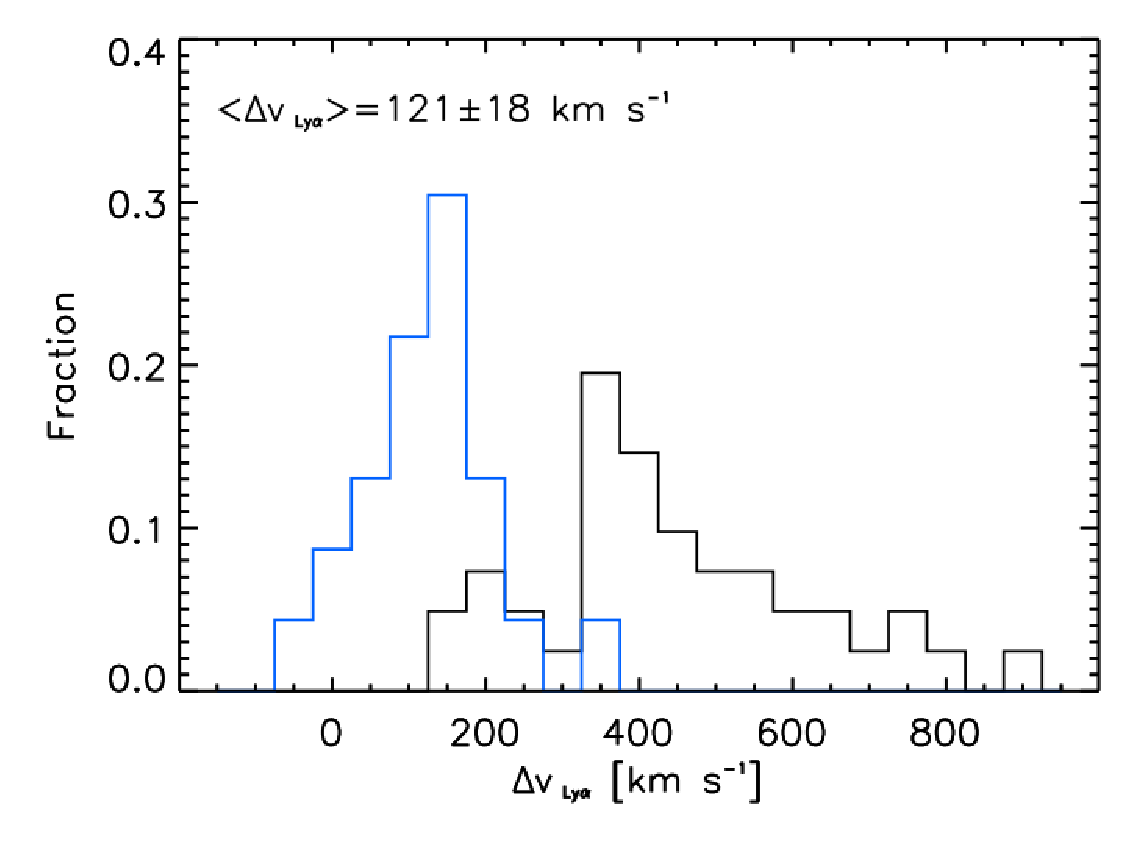
\includegraphics[scale=.5]{/Users/scarlata/PROJECTS/COS_Lya/delta_v.ps}
   \caption{Histogram of the velocity shifts between the 
\lya\ and \ha\ lines.}
   \label{fig:stack}
\end{figure*}

\begin{figure*}[]
   \centering
   \includegraphics[scale=.5]{/Users/scarlata/PROJECTS/COS_Lya/stack.ps}
   \caption{Composite spectrum from XXX galaxies.}
   \label{fig:stack}
\end{figure*}

In Figure~\ref{fig:spectra_full} we show the observed COS spectra
centered on the galaxy systemic velocity derived using the \ha\
emission line. The spectra are shown after a 9 pixels ($\sim$0.1\AA)
boxcar average. In two galaxies (GALEX1418$+$5259 and
GALEX0959$+$0149) the \lya\ line is very faint, and it is detected
only after a rather heavy boxcar smoothing ($\sim 0.7$\AA).

From the images shown in Figure~\ref{fig:images} we cans 
In Figures~\ref{fig:line_profiles} we show the profiles of the \lya\
emission lines. The vertical dashed line shows the expected wavelength
position of the \lya\ based on optical-lines redshift measurements.

Depending on the $S/N$ of the spectra the lines show a nice blue peak.

Figure~\ref{fig:histvel} shows the 

\subsection{Profile properties in various cases}

Let $x$ be :
\begin{equation}
x=\frac{\nu - \nu_0}{\Delta \nu_D};
\end{equation}

\noindent
where $\nu_D=V_{th}/c\nu_)$ is the Doppler frequency width.

\noindent
{\bf Homogeneous slab, monocromatic radiation} 
What determines the shape of the output spectrum in this case are the
temperature and the optical depth of the neutral medium.
For a dust-free slab, the profile is double peaked and simmetric
around $x=0$. The peak frequency in this case ($x_p$) depends on $T$
and $\tau_0$ (the optical depth at the line center),
with $x_p \sim \pm 0.88(a\tau_0)^1/3$. The more optically thick the
medium is the more the peaks are separated.

In the presence of dust, the profile does not change much.

{\bf Expanding infalling halos}
The \lya\ profiles resulting from a monochromatic source surroundes by
an expanding/infalling shell of gas are perfectly symmetric to
each other. Expanding halos present a red peak while infalling halos
show a blue peak.


\section{Radiative driven stellar winds}
Winds==> high density==> expnding material is opaque/optically thick
to scattering in many atominc spectral-line transitions.
\section{Dust Geometry and reddening}

\section{Discussion}

\section{Conclusions}

%\bibliographystyle{jphysiscsB} 
%\bibliographystyle{apj} 
%\bibliography{mybib}
\begin{thebibliography}{32}
\bibitem[{Atek} {et~al.}(2008)]{atek2008} Atek, H., Kunth, D., Hayes, M., Ostlin, G.,  Mas-Hesse, J. M. 2008, A\&A, 488, 491
\bibitem[{Atek} {et~al.}(2009)]{atek2009} Atek, H., Kunth, D.,  Schaerer, D. et al. 2009, ArXive e-prints 0906.5349
\bibitem[{Baldwin} {et~al.}(1981)]{baldwin1981} Baldwin, J. A., Phillips, M. M.,  Terlevich, R. 1981, PASP, 93, 5
\bibitem[{{Bruzual} \& {Charlot}(1993)}]{bruzual1993} Bruzual, A. G. \& Charlot, S. 1993, ApJ, 405, 538
\bibitem[{{Bruzual} \& {Charlot}(2003)}]{bruzual2003} Bruzual, G. \& Charlot, S. 2003, MNRAS, 344, 1000
\bibitem[{{Caplan} \& {Deharveng}(1986)}]{caplan1986} Caplan, J. \& Deharveng, L. 1986, A\&A, 155, 297
\bibitem[{Cardelli} {et~al.}(1989)]{cardelli1989} Cardelli, J. A., Clayton, G. C.,  Mathis, J. S. 1989, ApJ, 345, 245
\bibitem[{Carter} {et~al.}(2001)]{carter2001} Carter, B. J., Fabricant, D. G., Geller, M. J., Kurtz, M. J., \& McLean, B. 2001, ApJ, 559,606
\bibitem[{{Charlot} \& {Fall}(1993)}]{charlot1993} Charlot, S. \& Fall, S. M. 1993, ApJ, 415, 580
\bibitem[{Cowie} {et~al.}(2009)]{cowie2009} Cowie, L.L., Barger, A.J., Hu, E.M., 2009, ArXive e-prints 0909.0031
\bibitem[{Deharveng} {et~al.}(2008)]{deharveng2008} Deharveng, J.-M., Small, T.,  Barlow, T. A. et al. 2008, ApJ, 680, 1072
\bibitem[{Dijkstra} {et~al.}(2006)]{dijkstra2006} Dijkstra, M., Haiman, Z., \& Spaans, M. 2006, ApJ, 649, 14
\bibitem[{Finkelstein} {et~al.}(2008)]{finkelstein2008geom} Finkelstein, S. L., Rohads, J. E.,  Malhotra, S. et al. 2008, ApJ, 678, 655
\bibitem[{Finkelstein} {et~al.}(2009a)]{finkelstein2009} Finkelstein, S. L., et al., 2009, ApJ, 700, 276
\bibitem[{Finkelstein} {et~al.}(2009b)]{finkelsteinagn} Finkelstein, S. L., et al., 2009, ApJ, ArXive e-prints 0906.4554
\bibitem[{Giavalisco} {et~al.}(1996)]{giavalisco1996} Giavalisco, M., Koratkar, A., \& Calzetti, D. 1996, ApJ, 466, 831
\bibitem[{Hansen} {et~al.}(2006)]{hansen2006} Hansen, M. \& Oh, S. P. 2006, MNRAS, 367, 979
\bibitem[{Hayes} {et~al.}(2007)]{hayes2007} Hayes, M. et al. 2007, MNRAS, 382, 1465
\bibitem[{Kauffmann} {et~al.}(2003)]{kauffmann2003} Kauffmann, G. et al. 2003, MNRAS, 341, 33
\bibitem[{Kewley} {et~al.}(2001)]{kewley2001} Kewley, L. J. et al. 2001, ApJ, 556, 121
\bibitem[{{Laursen} \& {Sommer-Larsen}(2007)}]{laursen2007} Laursen, P. \& Sommer-Larsen, J. 2007, ApJ, 657, L69
\bibitem[{Mathis}(1972)]{mathis1972} Mathis, J. S. 1972, ApJ, 176, 651
\bibitem[{Miller} {et~al.}(2003)]{miller2003} Miller, C. J. et al. 2003, ApJ, 597, 142
\bibitem[{{Natta} \& {Panagia}(1984)}]{natta1984} Natta, A. \& Panagia, N. 1984, ApJ, 287, 228
\bibitem[{Neufeld}(1990)]{neufeld1990} Neufeld, D.~A. 1990, ApJ, 350, 216
\bibitem[{Neufeld}(1991)]{neufeld1991} Neufeld, D.~A. 1991, ApJ, 370, L85
\bibitem[{{Oke} \& {Gunn}(1982)}]{dbsp} Oke, J. B. \& Gunn, J. E. 1982, PASP, 94, 586
\bibitem[{Ostlin} {et~al.}(2008)]{ostlin2009} Ostlin, G. et al. 2008, ArXiv e-prints
\bibitem[{{Panagia} \& {Ranieri}(1973a)}]{panagia1973a} Panagia, N. \& Ranieri, M. 1973a, A\&A, 24, 219
\bibitem[{{Panagia} \& {Ranieri}(1973b)}]{panagia1973b} Panagia, N. \& Ranieri, M. 1973b, in Les N´ebuleuses Plan´etaires, 275–280
\bibitem[{Pengelly}(1964)]{pengelly1964} Pengelly, R. M. 1964, MNRAS, 127, 145
\bibitem[{Valls-Gabaud}(1993)]{vallsgabaud1993} Valls-Gabaud, D. 1993, ApJ, 419, 7
\bibitem[{Verhamme} {et~al.}(2006)]{verhamme2006} Verhamme, A., Schaerer, D., \& Maselli, A. 2006, A\&A, 460, 397
\bibitem[{York} {et~al.}(2000)]{sdss} York, D. G. et al. 2000, AJ, 120, 1579



\end{thebibliography}

\appendix
\begin{deluxetable}{lcccl} 
\tablecolumns{5} 
\tablewidth{0pc} 
\tablecaption{\lya\ properties} 
\tablehead{ 
\colhead{Galaxy}    & \colhead{\lya\ luminosity} &  \colhead{$\lambda_{B}$}   &  \colhead{$\lambda_{R}$}   & \colhead{Notes}\\
\cline{1-5} \\ 
\colhead{} & \colhead{erg s$^{-1}$}   &  \multicolumn{2}{c}{\AA} &\colhead{}}
\startdata 
GALEX1417+5228  & 1.38 $\pm$ 0.03 $\times 10^{42}$  & 1467.93 $\pm$ 0.01 & 1469.15 $\pm$ 0.01&      \\
GALEX0331-2814\tablenotemark{a} & 1.30 $\pm$ 0.05 $\times 10^{42}$  & \nodata & 1556.30 $\pm$ 0.10&      \\
GALEX0332-2801  & 0.39 $\pm$ 0.02 $\times 10^{42}$  & 1475.82 $\pm$ 0.01 & 1478.90 $\pm$ 0.01&      \\
GALEX1418+5307  & 0.53 $\pm$ 0.02 $\times 10^{42}$  & 1462.12 $\pm$ 0.01 & 1463.68 $\pm$ 0.03&      \\
GALEX0332-2811A  & 1.06 $\pm$ 0.02 $\times 10^{42}$  & \nodata & 1465.08 $\pm$ 0.01&      \\
GALEX1436+3459  & 0.38 $\pm$ 0.02 $\times 10^{42}$  & 1473.83 $\pm$ 0.01 & 1474.98 $\pm$ 0.01&      \\
GALEX1418+5259  & 0.04 $\pm$ 0.02 $\times 10^{42}$  & \nodata  & \nodata&      \\
GALEX1001+0233  & 1.83 $\pm$ 0.14 $\times 10^{42}$  & \nodata & 1682.10 $\pm$ 0.01&      \\
GALEX1437+3445  & 0.83 $\pm$ 0.07 $\times 10^{42}$  & \nodata & 1610.23 $\pm$ 0.01&      \\
GALEX1417+5305  & 0.31 $\pm$ 0.03 $\times 10^{42}$  & \nodata & 1541.07 $\pm$ 0.01&      \\
GALEX1436+3456  & 0.59 $\pm$ 0.04 $\times 10^{42}$  & \nodata & 1543.24 $\pm$ 0.01&      \\
GALEX0959+0149  & 0.02 $\pm$ 0.00 $\times 10^{42}$  & \nodata  & \nodata&      \\
GALEX0331-2811\tablenotemark{a} & 0.17 $\pm$ 0.01 $\times 10^{42}$  & \nodata & 1474.29 $\pm$ 0.10&      \\
GALEX0959+0151  & 0.29 $\pm$ 0.02 $\times 10^{42}$  & \nodata & 1521.75 $\pm$ 0.01&      \\
GALEX0330-2816  & 0.52 $\pm$ 0.04 $\times 10^{42}$  & 1555.92 $\pm$ 0.01 & 1558.40 $\pm$ 0.01&      \\
GALEX1420+5247  & 0.40 $\pm$ 0.03 $\times 10^{42}$  & 1520.95 $\pm$ 0.01 & 1523.22 $\pm$ 0.01&      \\
GALEX1717+5944  & 0.24 $\pm$ 0.01 $\times 10^{42}$  & \nodata & 1453.92 $\pm$ 0.01&      \\
GALEX0333-2821  & 0.37 $\pm$ 0.03 $\times 10^{42}$  & 1515.08 $\pm$ 0.01 & 1517.56 $\pm$ 0.01&      \\
GALEX1419+5315\tablenotemark{a} & 0.25 $\pm$ 0.02 $\times 10^{42}$  & 1535.93 $\pm$ 0.10 & 1536.80 $\pm$ 0.10&      \\
GALEX1418+5218  & 0.22 $\pm$ 0.02 $\times 10^{42}$  & \nodata & 1507.02 $\pm$ 0.01&      \\
GALEX1434+3532\tablenotemark{a} & 0.16 $\pm$ 0.01 $\times 10^{42}$  & 1453.15 $\pm$ 0.10 & 1454.12 $\pm$ 0.10&      \\
GALEX1000+0157  & 1.23 $\pm$ 0.05 $\times 10^{42}$  & 1535.20 $\pm$ 0.01 & 1538.83 $\pm$ 0.03&      \\
GALEX1423+5246  & 0.43 $\pm$ 0.07 $\times 10^{42}$  & 1632.31 $\pm$ 0.01 & 1634.03 $\pm$ 0.01&      \\
GALEX1420+5243  & 0.11 $\pm$ 0.01 $\times 10^{42}$  & \nodata & 1517.26 $\pm$ 0.01&      \\
GALEX1418+5217  & 0.07 $\pm$ 0.01 $\times 10^{42}$  & \nodata & 1508.37 $\pm$ 0.01&      \\
\enddata 
\tablenotetext{a}{Galaxy observed with MIRRORB}
\end{deluxetable}
\clearpage
\begin{figure}
\epsscale{1.}
\plotone{/Users/scarlata/PROJECTS/COS_Lya/images_COS.ps}
\caption{\label{fig:images} COS NUV images of the target galaxies. The
  circles show the position and size of the COS PSA aperture. For four
  galaxies an accurate position of the aperture could not be
  determined, and the aperture is not shown (see text for details).}
\end{figure}


\end{document}

